%! TEX program = xelatex

\documentclass[utf8]{gradu3}

\usepackage{graphicx}
\usepackage{csquotes}
\usepackage{amsmath,amssymb,amsthm}
\usepackage{biblatex}
\usepackage[bookmarksopen,bookmarksnumbered,linktocpage]{hyperref}

\addbibresource{sources.bib}

\title{Pro gradu -tutkielman tutkimussuunnitelma}
\translatedtitle{Master's thesis research plan}
\author{Mikael Myyrä}
\contactinformation{\texttt{mikael.b.myyra@jyu.fi}}
\supervisor{Sanna Mönkölä, Tuomo Rossi, Jonni Lohi}
\studyline{Teknis-matemaattinen mallintaminen}
\tiivistelma{-}
\abstract{-}
\avainsanat{
yleistetty differenssimenetelmä,
kontrollimenetelmä,
akustiikka,
simulointi
}
\keywords{
discrete exterior calculus,
exact controllability,
acoustics,
simulation
}

\begin{document}

\maketitle
\mainmatter
\sloppypar

\chapter{Johdanto}

Tutkimuksen aiheena on yleistetyn differenssimenetelmän
(engl. Discrete Exterior Calculus, DEC) ja kontrollimenetelmän
soveltaminen kaksiulotteiseen akustiikkasimulatioon.
DEC:ä käytetään simulointitehtävien paikka- ja aikadiskretointiin.
Kontrollimenetelmällä pyritään löytämään nopeasti lopullinen (ajassa jaksollinen) tila,
jota kohti simuloitu systeemi kehittyy ajan kuluessa.

Näitä menetelmiä on tutkittu suhteellisen vähän,
ja niillä on kiinnostavia ominaisuuksia
ratkaisun tarkkuuden ja tehokkuuden näkökulmista.
Tarkemmilla simulointimenetelmillä pystytään tekemään luotettavampia arvioita
todellisten systeemien käyttäytymisestä.
Tehokkaammilla menetelmillä puolestaan nopeutetaan iterointia
esim. rakenteiden suunnittelutyössä
ja toisaalta mahdollistetaan suurempien
ja monimutkaisempien systeemien simulointi
käytännöllisessä laskenta-ajassa.

Tämä on uusi sovelluskohde DEC:n ja kontrollimenetelmän yhdistelmälle,
joten tutkimuksesta saadaan uutta tietoa menetelmien käyttäytymisestä eri tehtävissä.

\chapter{Kirjallisuuskartoitus}

Kirjallisuuden haku alkoi tutkimusryhmän asiantuntijoilta saaduista avainlähteistä
ja niiden lähdeviitteistä.
Lisäksi tehtiin täydentävä haku Google Scholar -hakukoneella
avainsanoilla ''Discrete Exterior Calculus acoustics'' ja ''exact controllability''.

Menetelmä perustuu differentiaalimuotoihin, joiden teoriaa käsitellään
oppikirjoissa \parencite{abraham_manifolds_2012} ja \parencite{lee_introduction_2012}
sekä vähemmän formaalisti artikkelissa \parencite{blair_perot_differential_2014}
ja kurssimateriaalissa \parencite{crane_digital_2013}.
Muita akustiikkatehtävässä tarvittavia matemaattisia käsitteitä
käsitellään mm. artikkeleissa \parencite{lohi_whitney_2021},
\parencite{engquist_absorbing_1977}, \parencite{mur_finite-element_1993}
ja \parencite{plessix_review_2006} sekä luentomonisteessa \parencite{gillette_notes_2009}.

Kontrollimenetelmän matemaattista teoriaa käsitellään artikkeleissa
\parencite{glowinski_ensuring_1992}, \parencite{lasiecka_exact_1989},
\parencite{lasiecka_exact_1989}, \parencite{lions_exact_1988}
ja \parencite{bristeau_controllability_1998}.

DEC-menetelmä on yleistetty muoto tunnetusta Yeen \parencite*{yee_numerical_1966}
Finite Difference Time Domain (FDTD) -menetelmästä.
Yleistys mahdollistaa muut kuin koordinaattiakselien suuntaiset laskentaverkot
ja laskennan epäeuklidisissa avaruuksissa.
DEC:n esittelivät ensimmäistä kertaa Desbrun ym. \parencite*{desbrun_discrete_2005}.
Sitä on sovellettu mm. sähkömagnetiikkaan
\parencite{bossavit_discretization_2005,rabina_numerical_2014,rabina_efficient_2015,monkola_discrete_2022},
virtausdynamiikkaan \parencite{nitschke_discrete_2017},
Darcyn virtaukseen \parencite{hirani_numerical_2015}
sekä akustiikkaan ja elastodynamiikkaan \parencite{vandekerckhove_mimetic_2014}.
Artikkeleissa \parencite{rabina_generalized_2018} ja \parencite{rossi_systematisation_2021}
on kehitetty DEC:n pohjalta yhdistävää yleistä teoriaa useille erityyppisille aaltoilmiöille.

Tutkimusmenetelmien osalta sovellan konstruktiivisen tieteen \parencite{kacprzyk_constructive_2010}
ja suunnittelutieteen \parencite{hevner_design_2004} ajatuksia
sekä laskennallisen tieteen toistettavuuden periaatteita \parencite{stodden_best_2013}.

\chapter{Tutkimusaihe/tutkimuskysymys}

Ensisijainen tutkimuskysymys on,
miten DEC ja kontrollimenetelmä soveltuvat akustiikkatehtävän ratkaisuun.

Tätä tarkastellaan ainakin seuraavien konkreettisempien kysymysten kautta:
Miten tarkasti DEC toistaa tunnetun analyyttisen ratkaisun,
ja miten tämä riippuu käytetystä laskentaverkosta?
Kuinka nopeasti kontrollimenetelmä konvergoi
verrattuna tavanomaiseen ajasta riippuvaan ratkaisijaan?

\chapter{Tutkimusstrategia/metodi ja sen valintaperusteet}

Tutkimuksen tärkein tehtävä on simulointiohjelmiston rakentaminen.
Tämä on tekninen, konstruktiivinen tehtävä, johon on luontevaa soveltaa
suunnittelu- ja konstruktiivisen tieteen menetelmiä
sekä ohjelmistokehityksen yleisiä käytäntöjä.
Kehittämisessä pyritään maksimoimaan ohjelmiston testattavuus ja mitattavuus,
käytetään testausta ja mittausta toimivuuden arviointiin
sekä käytetään versionhallintaa välitulosten tallentamiseen.
Toistettavuuden ja avoimuuden takaamiseksi kaikki tutkimuksessa toteutettu ohjelmakoodi
julkistetaan avoimella lisenssillä GitHub-palvelussa.

Kehittämisen helpottamiseksi simulointikokeet on suunniteltu siten,
että järjestelmän osia pystytään testaamaan erillään toisistaan.
Aluksi kehitetään tilayhtälön ratkaisija, jota testataan sille suunnitelluilla kokeilla.
Kun tilayhtälön ratkaisija on todettu toimivaksi, kehitetään kontrollimenetelmän ratkaisija,
jota käytetään varsinaisen tutkimustehtävän ratkaisemiseen.

\chapter{Aineiston keruu}

Tutkimukseen ei tarvita ihmisosallistujia.
Aineisto saadaan toteutettujen simulointikokeiden tuloksista,
ja sen käsittely on koekohtaista.
Pääsääntöisesti kokeen tulokset voidaan ilmoittaa sellaisenaan tutkimustuloksina.

\chapter{Tulokset}

Tähän mennessä on saatu toteutettua tilayhtälön ratkaisija
ja kaksi testitapausta.
Ensimmäinen testitapaus on yksinkertainen tasoaalto,
jonka analyyttinen ratkaisu tunnetaan (kuva \ref{acc_test}).
Ratkaisijan tarkkuutta testattiin vertaamalla saatuja tuloksia
tunnettuun ratkaisuun.

Toinen testitapaus (kuva \ref{scatterer}) mallintaa ympyrän muotoista kappaletta,
johon osuu edellistä tehtävää vastaava tasoaalto.
Ratkaistaan tästä syntyvä sironnut aalto.

Kontrollimenetelmästä ei ole vielä saatu tuloksia.

\begin{figure}[t]
  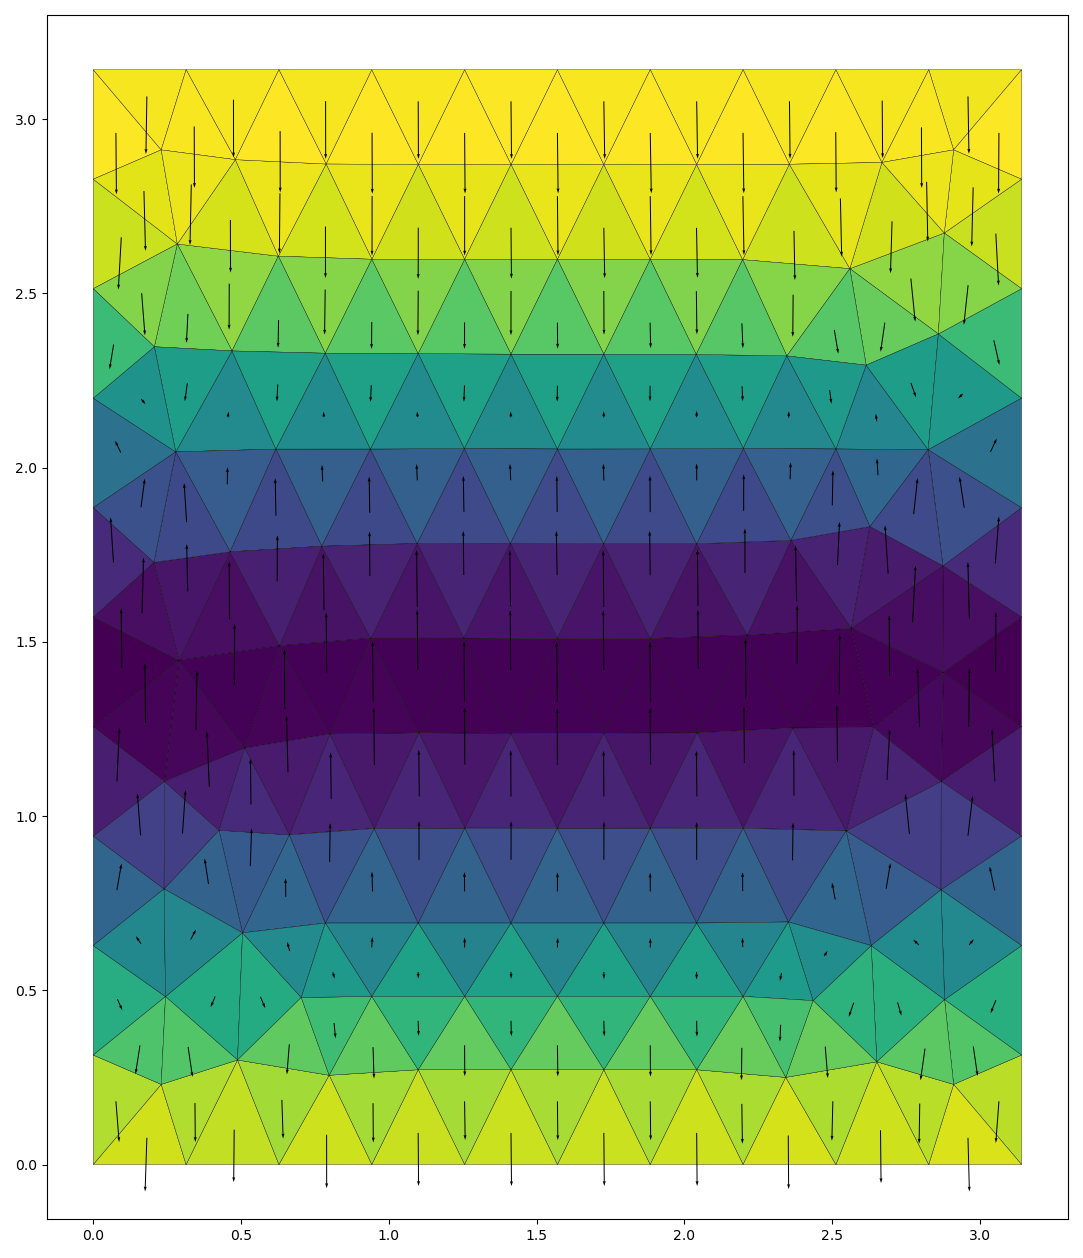
\includegraphics[width=0.5\textwidth]{research_plan/accuracy_test_wave.png}
  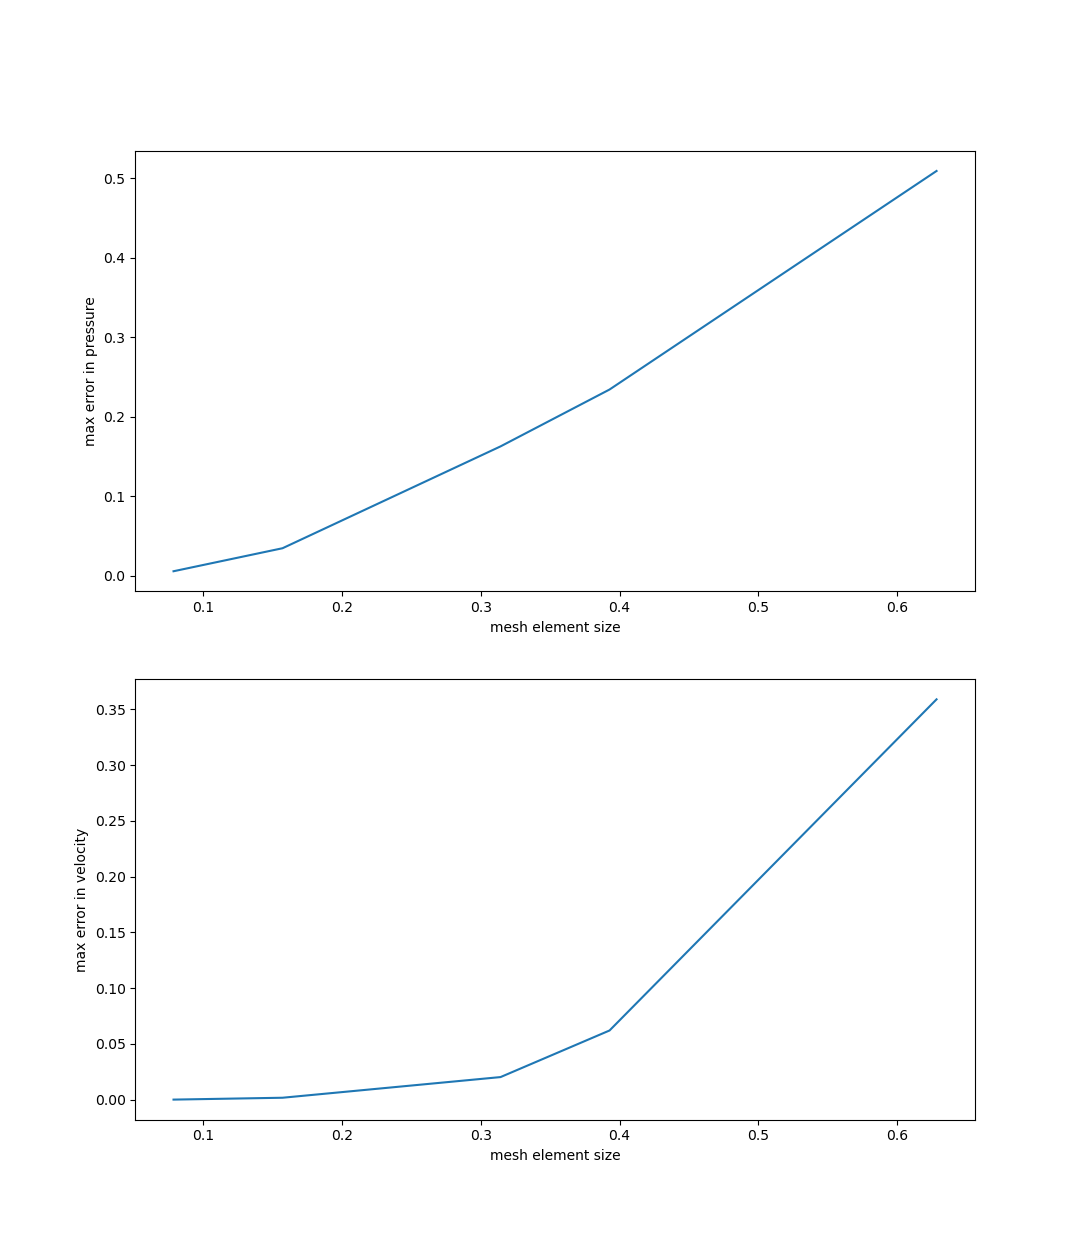
\includegraphics[width=0.5\textwidth]{research_plan/accuracy_test_sizes.png}
  \caption{
  \label{acc_test}
  Vasen kuva: Tasoaalto, jolla testataan tilayhtälön ratkaisijan tarkkuutta.
  Väri kuvaa aallon akustista painetta ja nuolet värähtelevien hiukkasten nopeutta.
  Oikea kuva: Tasoaallon suurin virhe verrattuna tunnettuun ratkaisuun
  ja sen riippuvuus laskentaverkon elementtien koosta.
  }
\end{figure}

\begin{figure}[h]
  \centering
  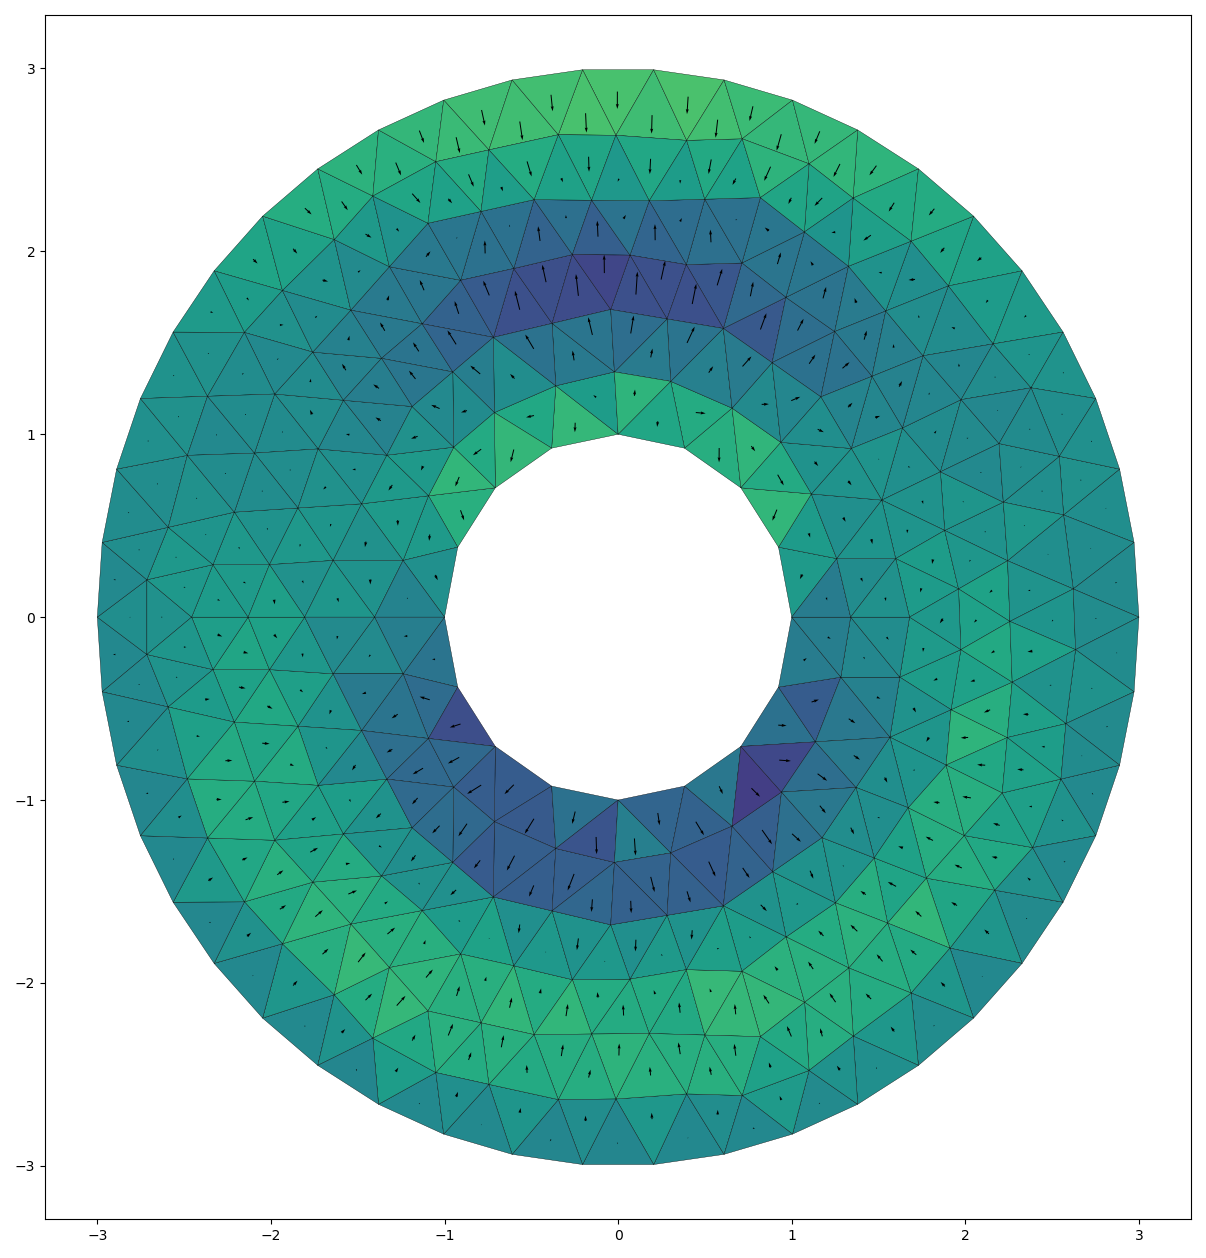
\includegraphics[width=0.5\textwidth]{research_plan/scatterer.png}
  \caption{
    \label{scatterer}
    Keskellä olevasta ympyräkappaleesta sironnut aalto.
  }
\end{figure}

\chapter{Johtopäätökset}

Tähän mennessä saatujen tulosten perusteella
DEC vaikuttaa soveltuvan hyvin akustiikkasimulaatioihin.
Tilayhtälön ratkaisija on todettu stabiiliksi,
ja sen tarkkuus käyttäytyy odotetulla tavalla.
Tarkkuutta saadaan todennäköisesti vielä parannettua
käyttämällä hyödyksi olettamusta ratkaisun aikaharmonisuudesta.

Aikaisemman tiedon perusteella on odotettavissa,
että kontrollimenetelmä nopeuttaa konvergenssiä huomattavasti
erityisesti monimutkaisen geometrian tapauksissa.

\printbibliography

\end{document}
